%\documentclass{hitec}
\documentclass{myhitec}
\usepackage[UTF8]{ctex}
\usepackage{fontspec}
\usepackage[dvipsnames]{xcolor}
\usepackage{amsmath}
\usepackage{array}
\usepackage{graphicx}
\usepackage{longtable}
\usepackage{booktabs}  %用于美观表格线宽
\usepackage{multirow}  %用于跨行表
\usepackage{tabularx}  %定义表格宽度
\usepackage{float}
\usepackage{indentfirst}
\usepackage{bibentry}
%\usepackage[linkcolor=gray!40!black]{hyperref}
\usepackage[colorlinks,urlcolor=blue!50!black,linkcolor=blue!50!black,anchorcolor=blue,citecolor=blue!50!black,CJKbookmarks=True]{hyperref}
\usepackage{tcolorbox}
\usepackage{hyperref} % This line is readily ommited of it makes trouble
\tcbuselibrary{breakable,listings,skins,fitting}
\usepackage{newenviron}

%\usepackage{changepage}
%\begin{adjustwidth}{2cm}{1cm}
%\end{adjustwidth}

%==========================================
% Latex 命令环境设置
%==========================================

%==========================================
% 字体设置
%==========================================
%\newfontfamily{\monoca}{Monaco}
\newfontfamily{\monoca}{Microsoft YaHei}
% \setCJKmainfont{FandolSong}
% \setmainfont{FiraSans-Light}
% \setsansfont{FiraSans-Hair}
% \setmonofont{FiraMono-Regular}

\setCJKmainfont{Microsoft YaHei}
% \setmainfont{Microsoft YaHei}
% \setsansfont{Microsoft YaHei}
% \setmonofont{Microsoft YaHei}

\setmainfont{Consolas}
\setsansfont{Consolas}
\setmonofont{Consolas}


%==========================================
% 自定义命令设置
%==========================================
\newcommand{\urllink}[2]{\href{#1}{#2}}

\newcommand{\HT}{\textsc{\raisebox{0.1em}{H}\raisebox{-0.1em}{I}%
	\raisebox{0.1em}{T}\raisebox{-0.1em}{E}\raisebox{0.1em}{C} }}

\newtheorem{thm}{定理}
\newcommand\degree{^\circ}

\newtcbox{\emphasizebox}[1][blue]{enhanced,on line,%drop fuzzy shadow,
arc=2pt,outer arc=2pt,colback=#1!5!white,colframe=#1!50!black,
boxsep=0pt,left=3pt,right=3pt,top=1pt,bottom=1pt,
colupper=blue!50!black,fit basedim=10pt,
boxrule=0.1pt,bottomrule=0.1pt,toprule=0.1pt,nobeforeafter}

%==========================================
% 自定义lsting设置
%==========================================
\newtcblisting{messagebox}{%
breakable,
left=3mm,
listing only,
boxrule=0.2mm,
colback=gray!5,
fontupper=\monoca,colupper=red!50!black,
coltext=black
}%

\newtcblisting{commandbox}{%
breakable,
left=3mm,
listing only,
boxrule=0.2mm,
colback=black,
fontupper=\monoca,colupper=red!50!black,
coltext=green
}%

\newtcblisting{codeout}{%
breakable,
left=3mm,
boxrule=0.2mm,
colback=gray!5,
fontupper=\monoca,colupper=red!50!black,
coltext=black
}%

%\lstset{
    % numbers=left,
    % %numberstyle={\color{lightgray}},
    % numberstyle={\color{green}},
    % backgroundcolor={\color[RGB]{41, 47, 51}}, %背景颜色
    % basicstyle={\color[RGB]{208, 214, 219}}, %普通字符串颜色
    % stringstyle={\color[RGB]{0, 128, 0}}, %字符串颜色
    % keywordstyle={\color[RGB]{101, 140, 230}}, %关键词颜色
    % commentstyle={\color{gray}}, %注释颜色
    % frame=none, %无边框
    % breaklines=true, %自动分行
    % language={[ANSI]C},
    % captionpos=b,
% }

\lstnewenvironment{myccode}[1][]
{\lstset{
    numbers=left,
    %numberstyle={\color{lightgray}},
    %frame=none, %无边框
    frame=lines, %上下线
    %frame=single, %边框
    language={[ANSI]C},
    breaklines=true, %自动分行
    %keywordstyle={\color{blue}}, %关键词颜色
    %stringstyle={\color{orange}}, %字符串颜色
    %stringstyle={\color{magenta}}, %字符串颜色
    %commentstyle={\color{green}}, %注释颜色
    %basicstyle={\color[black]}, %普通字符串颜色
    %captionpos=b,
    #1
        }
}
{}

%==========================================
% 标签格式
%==========================================
\hypersetup{
    colorlinks=true,
    bookmarksnumbered=true,
    pdftitle={My LaTeX2e note},
    pdfkeywords={LaTex, note},
}

%==========================================
% 摘抄格式
%==========================================
\newenvironment{literbox}
%{\begin{messagebox}
{\begin{quote}\zihao{-4}\kaishu
%{\zihao{-3}\kaishu
}
%{\end{messagebox}}
{\end{quote}}
%{}

%==========================================
% 图片路径
%==========================================
\graphicspath{{figure/}, 
{005_protocol_note/bt_picture/}, 
{009_soft_install_note/gvim_install_picture/}, 
{008_system_work_note/system_note_picture/}, 
}

%==========================================
% 水印
%==========================================
%\usepackage{draftwatermark}
%\SetWatermarkText{Zero Note} % the Text
%\SetWatermarkLightness{0.9} % the lightness from 0 to 1, default 0.8
%\SetWatermarkScale{1.0} % the scale, default 1.2


%==========================================
% 首页信息
%==========================================
\title{BR30 TDM测试环境说明}
\author{莫志烨}
\company{杰理科技-固件五部}
\confidential{\textbf{-- 非限制发布 --}}

%==========================================
% 开始排版
%==========================================
\begin{document}
\begin{titlepage}
\pdfbookmark[1]{标题页}{title}
\maketitle
%这是一篇关于\LaTeX 的文档,风格使用 \HT 。
\end{titlepage}

%\begin{abstract}
%本文说明如何用\LaTeX{}模板撰写报告。
%
%\end{abstract}
%提示:获取本文档的最新版本比现在开始阅读更重要。
%本文的最新版本见于:\url{https://git.coding.net/yangdawei/git.git}
\pdfbookmark[1]{目录}{contents}
\tableofcontents
\newpage
\newpage

%==========================================
% 图片路径
%==========================================
\graphicspath{{figure/},
{002_tdm_note/figure/},
}

%==========================================
% 章节内容
%==========================================
\section{TDM测试环境说明}
\subsection{关于测试环境相关文件}
\begin{itemize}
\item 服务器SDK工程,SDK工程路径:
\begin{messagebox}
/230common/mozhiye/BR30/br30_tdm_test_env_20200819
\end{messagebox}
\item 下载目录:
\begin{messagebox}
BR30_tdm_test_download.zip
\end{messagebox}
\item 骨传导传感器\myurlfootnote{https://www.st.com/resource/en/datasheet/lis25ba.pdf}{LIS25BA规格书};
\end{itemize}

\subsection{关于测试环境相关驱动文件组成}
\begin{itemize}
\item 传感器驱动文件:SDK/apps/common/device/gSensor/lis25ba.c
\item TDM接口驱动文件:SDK/lib/media/media\_new/cpu/br30/audio\_link.c
\item 修改数据接收方式头文件:SDK/include\_lib/driver/cpu/br30/asm/tdm\_test.h
\end{itemize}

\subsection{关于SDK修改}
由于ALINK接收数据位宽的限制(最大24bit),因此同一时刻只能接收传感器输出的X,Y,Z轴数据的其中两个轴数据,修改接收不同轴数据,需修改tdm\_test.h文件,选择需要接收的数据;
\begin{myccode}[caption={tdm\_test.h}]
#ifndef _TDM_TEST_H_
#define _TDM_TEST_H_

//===========================================//
//              接收TDM数据选择:二选一      //
//===========================================//
#define TDM_GET_X_Y_AXIS_DATA 		//选择接收X, Y数据
//#define TDM_GET_X_Z_AXIS_DATA     //选择接收X, Z数据

#define TDM_PUT_RAW_DATA

#endif /* #ifndef _TDM_TEST_H_ */
\end{myccode}

修改该文件后需要make工程并更新固件到小机,重新上电接收数据;


\subsection{关于串口数据接收工具使用}
\emphasizebox{SerialReadData.exe}工具可以将接收到的数据以文件的形式存储,使用步骤如下:
\begin{itemize}
\item 打开下载目录下serial tool/SerialReadData.exe工具;
\begin{figure}[H]
\centering
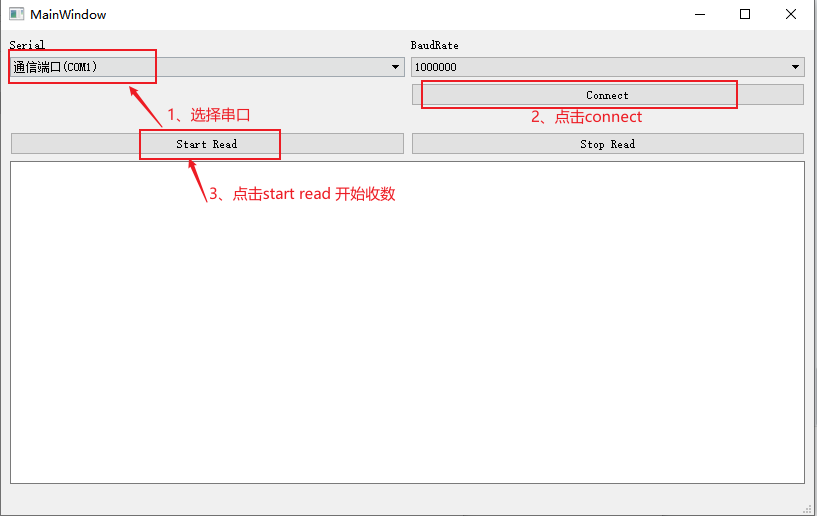
\includegraphics[scale=0.7]{firgure1.png}
\caption{打开串口接收工具}
\end{figure}

\item 重新上电BR30小板,工具显示框显示found flag, start write file表示开始收数;
\begin{figure}[H]
\centering
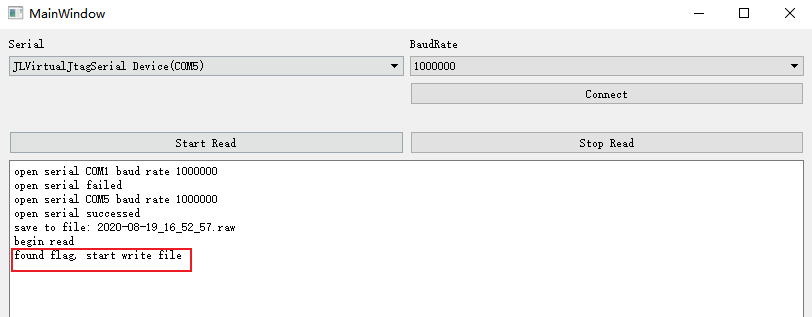
\includegraphics[scale=0.7]{firgure2.png}
\caption{开始接收数据}
\end{figure}

\item 停止收数,点击Stop Read;
\begin{figure}[H]
\centering
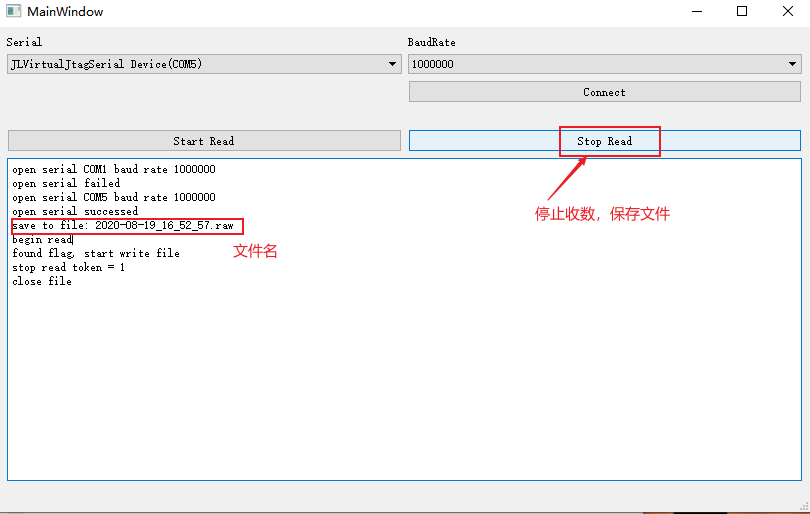
\includegraphics[scale=0.7]{firgure3.png}
\caption{停止接收数据}
\end{figure}

\item 打开保存的文件查看数据,文件开头4byte数据固定为字符串“abc”,分析数据时可不用理会,数据存储方式是X,Y或者X,Z轴数据交错存放:
\begin{figure}[H]
\centering
%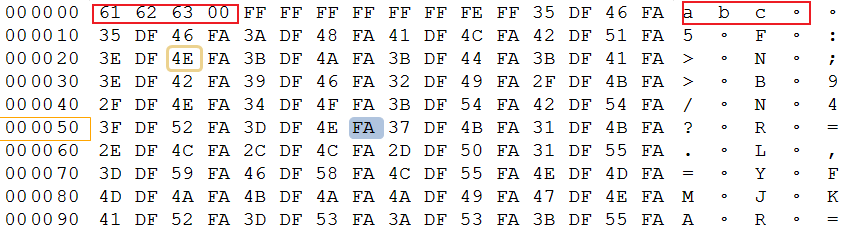
\includegraphics[height=8cm, width=16cm]{firgure4.png}
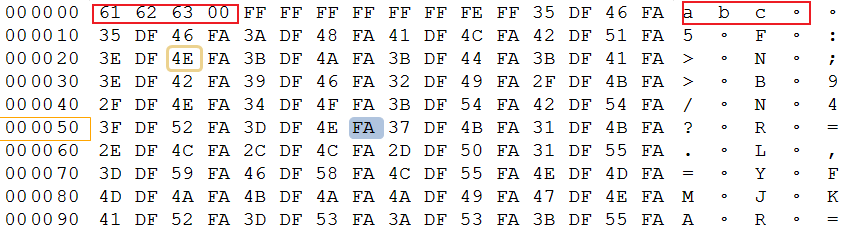
\includegraphics[scale=0.7]{firgure4.png}
\caption{检查接收数据}
\end{figure}


\end{itemize}




\end{document}


